% Richiede \usepackage{booktabs}, \usepackage{amsmath} e \usepackage{graphicx}
% nel preambolo di main.tex (le stesse dipendenze di
% fairmind_llm_benchmark_methodology.tex, con l'aggiunta di graphicx per le
% figure). Includila con \input{...} dove preferisci nel documento.
%
% Le tre figure referenziate sotto vivono in ./figures/ relativamente a
% questo file: se main.tex non imposta \graphicspath{{documenti_latex/figures/}}
% o equivalente, aggiusta i percorsi negli \includegraphics.

\section{Benchmark multi-dataset FairMind vs LLM}
\label{sec:multi-dataset-benchmark}

\subsection*{Obiettivo}

Il confronto descritto in \S\ref{sec:fairmind-llm-methodology} e \S\ref{sec:confronto-finale} riguarda un solo dataset (Adult Income). Questa sezione estende lo stesso protocollo di benchmark a \textbf{10 dataset reali} tra quelli disponibili in \texttt{data/processed/} (\texttt{notebooks/soldani\_task/2\_4\_benchmark\_multi\_dataset.ipynb}), per verificare se il pattern di accuratezza osservato su Adult --- LLM affidabile su TV e IE, meno affidabile su TE e DE, inutilizzabile su SE --- sia una propriet\`a del dataset specifico o si generalizzi a domini diversi (reddito, credito, recidiva penale, sanit\`a, istruzione).

\subsection*{Metodologia}

Lo schema resta lo Standard Fairness Model $X \to W \to Y$ con confondente $Z$ (Ple\v{c}ko e Bareinboim, 2024) gi\`a descritto in \S\ref{sec:fairmind-llm-methodology}, applicato per\`o a 10 configurazioni distinte (Tabella~\ref{tab:multi-config}), una per dataset. Per ciascun dataset FairMind stima la Bayesian Network e calcola i cinque effetti per inferenza esatta; lo stesso prompt a tabelle pre-aggregate viene inviato al LLM (Qwen2.5, servito via \texttt{llama.cpp} sullo stesso endpoint persistente usato negli esperimenti precedenti), con binning esplicito per i mediatori continui (es. \texttt{hours-per-week}, \texttt{priors\_count}, \texttt{ugpa}).

Esecuzione: notebook eseguito in automatico su Thor tramite \texttt{sbatch run\_benchmark\_multi.sbatch} (job Slurm 45178, 21 luglio 2026). Una nota tecnica rilevante per la riproducibilit\`a: il limite di completamento del LLM (\texttt{max\_tokens}) \`e stato alzato da 4096 a 8192 token in \texttt{src/llm.py} dopo che le prime due esecuzioni del notebook fallivano sistematicamente sui dataset con confondenti ad alta cardinalit\`a (\texttt{diabetes\_130}: 10 fasce et\`a $\times$ 3 fasce ricovero = 30 combinazioni $(z,w)$; \texttt{law\_bar\_pass}: 20; \texttt{oulad}: 25) --- il prompt chiede al modello di mostrare il calcolo passo-passo per ogni combinazione, e per questi dataset il testo generato superava 4096 token \emph{prima} di raggiungere il blocco \texttt{FINAL\_JSON}, producendo un output troncato e non parsabile.

\begin{table}[htbp]
\centering
\resizebox{\ifdim\width>\textwidth\textwidth\else\width\fi}{!}{%
\begin{tabular}{lllll r}
\toprule
Dataset & $X$ (protetto) & $x_0 \to x_1$ & $W$ (mediatore) & $Z$ (confondente) & $n$ \\
\midrule
adult & S2\_gender & Female$\to$Male & hours-per-week & education & 48\,842 \\
census\_income\_kdd & S1\_sex & Female$\to$Male & weeks\_worked\_in\_year & education & 200\,000 \\
bank\_marketing & S2\_marital & single$\to$married & housing & education & 40\,004 \\
compas & S1\_race & Caucasian$\to$Afr.-Am. & priors\_count & age\_cat & 6\,150 \\
diabetes\_130 & S1\_gender & Female$\to$Male & time\_in\_hospital & age & 101\,763 \\
german\_credit & S2\_Sex & Female$\to$Male & Length of employm. & Occupation & 1\,000 \\
law\_bar\_pass & S2\_race & Other$\to$White & ugpa & fam\_inc & 20\,512 \\
oulad & S1\_gender & F$\to$M & studied\_credits & highest\_education & 31\,482 \\
student\_mat & S2\_sex & F$\to$M & studytime & Medu & 395 \\
student\_por & S2\_sex & F$\to$M & studytime & Medu & 649 \\
\bottomrule
\end{tabular}%
}
\caption{Configurazione SFM per ciascuno dei 10 dataset benchmark.}
\label{tab:multi-config}
\end{table}

\subsection*{Risultati aggregati}

FairMind completa la stima e il calcolo dei 5 effetti in 11--12 millisecondi indipendentemente dal dataset (anche per \texttt{census\_income\_kdd}, 200\,000 righe). Il LLM impiega invece tra 21.7\,s (\texttt{adult}) e 82.2\,s (\texttt{law\_bar\_pass}) per risposta, per un totale di 478\,s e 69\,300 token su 10 chiamate --- circa 40\,000--70\,000 volte pi\`u lento di FairMind a seconda del dataset.

\begin{table}[htbp]
\centering
\resizebox{\ifdim\width>\textwidth\textwidth\else\width\fi}{!}{%
\begin{tabular}{lrr}
\toprule
Effetto & Errore relativo mediano & Segno concorde con FairMind \\
\midrule
TV & 0.2\% & 90\% \\
TE & 4.7\% & 90\% \\
DE & 94.6\% & 90\% \\
IE & 99.3\% & 60\% \\
SE & 309.7\% & 40\% \\
\bottomrule
\end{tabular}%
}
\caption{Errore relativo mediano e concordanza di segno per effetto, aggregati sui 10 dataset (50 confronti totali). L'errore mediano \`e usato al posto della media perch\'e alcuni confronti su SE hanno errore relativo di diverse centinaia per cento e distorcerebbero la media.}
\label{tab:multi-per-effect}
\end{table}

\begin{table}[htbp]
\centering
\resizebox{\ifdim\width>\textwidth\textwidth\else\width\fi}{!}{%
\begin{tabular}{lrr}
\toprule
Dataset & Errore assoluto medio & Errore relativo medio \\
\midrule
bank\_marketing & 0.0517 & 189.2\% \\
adult & 0.0400 & 44.3\% \\
compas & 0.0383 & 98.8\% \\
german\_credit & 0.0346 & 141.7\% \\
census\_income\_kdd & 0.0264 & 221.4\% \\
student\_mat & 0.0238 & 96.0\% \\
student\_por & 0.0217 & 127.2\% \\
law\_bar\_pass & 0.0096 & 30.2\% \\
oulad & 0.0050 & 103.0\% \\
diabetes\_130 & 0.0035 & 152.5\% \\
\bottomrule
\end{tabular}%
}
\caption{Errore medio per dataset, aggregato sui 5 effetti causali.}
\label{tab:multi-per-dataset}
\end{table}

\begin{figure}[htbp]
  \centering
  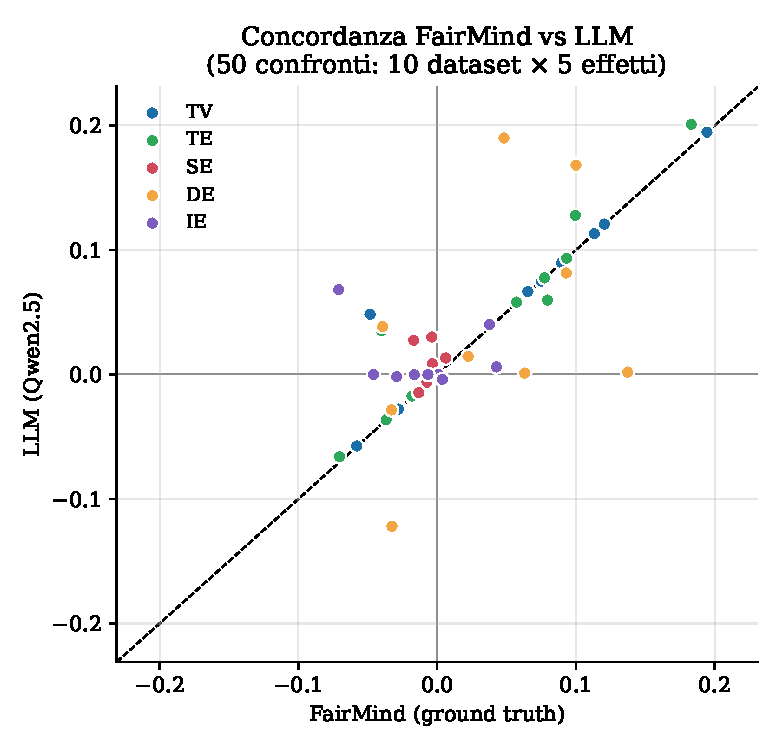
\includegraphics[width=0.68\linewidth]{figures/fig_scatter_fairmind_vs_llm.pdf}
  \caption{Valore FairMind (asse $x$) contro valore LLM (asse $y$) per tutti i 50 confronti (10 dataset $\times$ 5 effetti), colorati per tipo di effetto. La linea tratteggiata \`e la bisettrice $y=x$: i punti su TV/TE (blu/verde) vi si allineano da vicino, mentre SE (rosso) e IE (viola) sono dispersi e spesso nel quadrante opposto rispetto all'origine, cio\`e con segno invertito.}
  \label{fig:scatter}
\end{figure}

\begin{figure}[htbp]
  \centering
  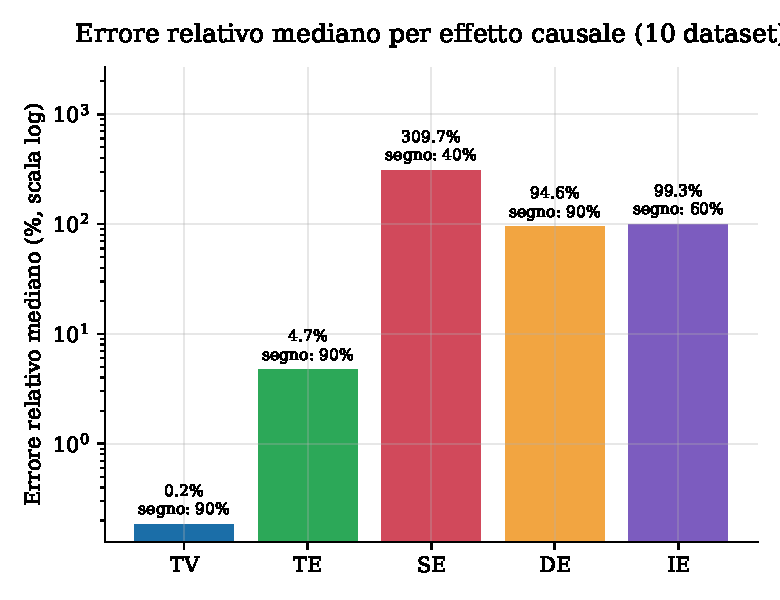
\includegraphics[width=0.68\linewidth]{figures/fig_median_rel_error_per_effect.pdf}
  \caption{Errore relativo mediano per effetto causale (scala log, 10 dataset), con percentuale di concordanza di segno annotata su ciascuna barra.}
  \label{fig:median-error}
\end{figure}

\begin{figure}[htbp]
  \centering
  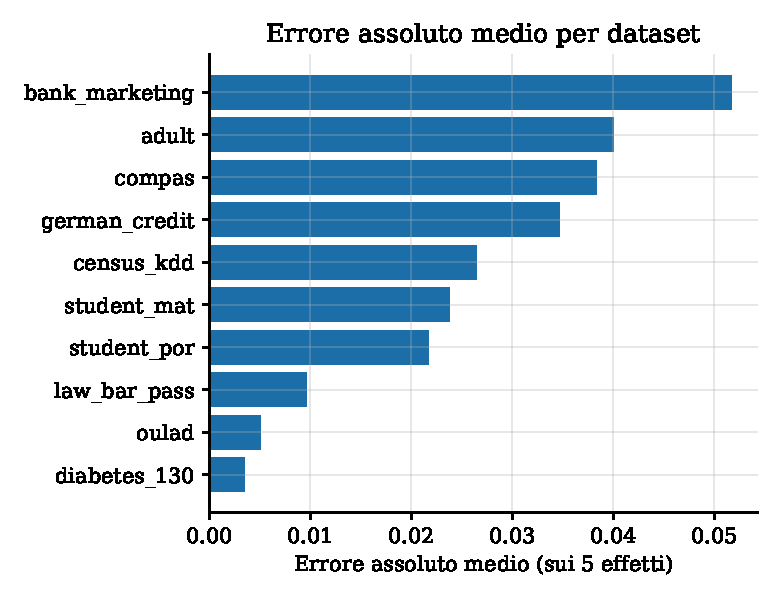
\includegraphics[width=0.68\linewidth]{figures/fig_mean_abs_error_per_dataset.pdf}
  \caption{Errore assoluto medio (sui 5 effetti) per dataset, ordinato.}
  \label{fig:abs-error-dataset}
\end{figure}

\subsection*{Analisi}

\begin{itemize}
  \item \textbf{La gerarchia TV $\approx$ TE $\ll$ DE $\approx$ IE $\ll$ SE osservata su Adult si conferma su tutti i 10 dataset.} Non era scontato: il pattern singolo poteva dipendere da caratteristiche specifiche di Adult (es. la particolare distribuzione di \texttt{hours-per-week}). Su 50 confronti indipendenti in 5 domini diversi l'ordine di difficolt\`a per il LLM resta lo stesso: TV e TE, calcolabili con poche operazioni dirette sulle tabelle 1 e 3, restano affidabili (errore mediano 0.2\% e 4.7\%); DE e IE, che richiedono sommare fino a 30 termini $(z,w)$, degradano fortemente (errore mediano attorno al 95--99\%); SE, differenza tra due quantit\`a vicine (TV$-$TE), resta la metrica pi\`u instabile (309.7\%).

  \item \textbf{Novit\`a rispetto al confronto singolo: la concordanza di segno.} Il dataset singolo non permetteva di distinguere se l'errore alto su SE/IE fosse "solo" di magnitudine o anche di direzione. Con 10 dataset emerge che per TV, TE e DE il LLM indovina il segno nel 90\% dei casi (9/10), ma per IE solo nel 60\% e per SE nel 40\% --- peggio del lancio di una moneta. Questo significa che per SE il LLM non \`e utilizzabile nemmeno a livello qualitativo (non si pu\`o nemmeno dire in modo affidabile se l'effetto spurio favorisca $x_0$ o $x_1$), un limite pi\`u severo del semplice "errore relativo alto".

  \item \textbf{Anomalia su \texttt{bank\_marketing}: segno invertito su TV, TE e DE.} \`E l'unico dataset in cui tre effetti su cinque (non solo quelli gi\`a fragili) hanno segno opposto a FairMind pur con magnitudine simile (es. TV: $-0.0483$ vs $+0.0483$). Un'ipotesi plausibile \`e che il modello abbia calcolato $x_0 - x_1$ invece di $x_1 - x_0$: la coppia \texttt{single}/\texttt{married} \`e semanticamente meno familiare, nei dati di addestramento del modello, come coppia "protetta/riferimento" rispetto a coppie pi\`u comuni come genere o razza, che potrebbero aver reso il modello meno attento a rispettare l'ordine $x_0, x_1$ dichiarato nel prompt. Resta un'ipotesi, non verificata: andrebbe confermata rileggendo la traccia di ragionamento completa salvata in \texttt{benchmark\_results/multi\_dataset/bank\_marketing\_*.json}.

  \item \textbf{La dimensione del dataset non sembra un fattore dominante.} \texttt{census\_income\_kdd} (200\,000 righe) ha errore relativo medio pi\`u alto (221\%) di \texttt{student\_mat} (395 righe, 96\%) o \texttt{german\_credit} (1\,000 righe, 142\%). \`E plausibile perch\'e sia FairMind sia il prompt al LLM operano gi\`a su probabilit\`a condizionali aggregate, non sui dati grezzi: una volta aggregate, tabelle da dataset grandi o piccoli hanno dimensione testuale comparabile nel prompt.

  \item \textbf{N\'e tempo di risposta n\'e token totali predicono l'accuratezza.} \texttt{law\_bar\_pass} \`e il pi\`u lento (82.2\,s) ma tra i pi\`u accurati (errore medio 30.2\%); \texttt{bank\_marketing} \`e relativamente veloce (43.9\,s, solo 4\,719 token) ma il pi\`u impreciso (189.2\%) e l'unico con segni invertiti. Un ragionamento pi\`u lungo o verboso non si traduce in un risultato pi\`u corretto in questo esperimento.
\end{itemize}

\subsection*{Conclusioni}

Il confronto su 10 dataset conferma, con un campione molto pi\`u ampio, quanto osservato sul solo Adult Income: FairMind resta l'unico riferimento affidabile per tutti e cinque gli effetti causali, con un costo computazionale (millisecondi) ordini di grandezza inferiore a quello del LLM (decine di secondi). Il LLM pu\`o fungere da "calcolatore causale" plausibile solo per TV e TE (errore mediano sotto il 5\%, segno corretto 9 volte su 10), mentre per DE e IE l'errore mediano supera il 90\% e per SE il segno stesso non \`e affidabile pi\`u della met\`a delle volte. Questo pattern \`e stabile attraverso domini molto diversi tra loro (reddito, marketing bancario, recidiva penale, sanit\`a, credito, istruzione), il che rafforza --- su una base empirica pi\`u solida di un singolo dataset --- l'ipotesi di tesi che l'inferenza causale formale debba restare il motore di calcolo per un'analisi di fairness rigorosa, riservando al LLM un ruolo di interprete dei risultati gi\`a calcolati piuttosto che di calcolatore diretto degli effetti pi\`u complessi (DE, IE, SE).
